\appendix
\chapter{Tuning auf Ihrem ToM+ (Twizy-cfg)}
\label{apx:tuning}

\section{Was ist Twizy-cfg?}

\href{http://github.com/dexterbg/Twizy-Cfg}{Twizy-Cfg} ist eine \textbf{Open-Source}, leichtgewichtige Konfigurations-Shell, die für den im Renault Twizy verbauten SEVCON
Gen4-Motorcontroller entwickelt wurde. Sie wurde von \href{https://github.com/dexterbg}{dexterbg} entwickelt.
Das Tool wurde für den Betrieb auf Arduino-Mikrocontrollern mit einem MCP2515-SPI-CAN-Bus-Modul entwickelt
und bietet Hardware-Hackern, Technikern und EV-Enthusiasten eine direkte
Kommandozeilenschnittstelle zur Interaktion mit dem Antriebssystem des Fahrzeugs über den standardmäßigen
\textbf{OBD-II-Diagnoseanschluss}.\\

Im Kern fungiert Twizy-cfg als Brücke zwischen \textit{High-Level}-Makrobefehlen und \textit{Low-Level}
CANopen-SDO-Registeroperationen. Dadurch ermöglicht es eine präzise Abstimmung und
Überwachung des Antriebsstrangs und bietet unter anderem folgende Möglichkeiten:\\

\begin{itemize}
    \item Anpassung des Fahrprofils: Einstellung wichtiger Leistungsparameter wie maximale Leistung, Drehmomentbegrenzungen, Höchstgeschwindigkeit und Beschleunigungsrampen.
    \item Energiemanagement: Feinabstimmung der Energierückgewinnung beim Ausrollen und Bremsen, um Reichweite und Bremswirkung auszubalancieren.
    \item Profilverwaltung: Speichern, Laden und Wiederherstellen benutzerdefinierter Leistungsprofile direkt im bzw. aus dem EEPROM des Arduino.
    \item Diagnose \& Low-Level-Zugriff: Ausführen von rohen CANopen-Befehlen und grundlegenden OBD-II-Diagnoseanfragen zur Untersuchung von Controller-Zuständen und Firmware-Versionen.
\end{itemize}
\  \\
Dieser Anhang beschreibt, wie ToM+ eine spezielle Partition mit der oben genannten
Software verwalten kann, die für den Betrieb auf dem ESP32-Board (ToM+-Chip) angepasst wurde.


\section{Voraussetzungen}

\textbf{HINWEIS!} Ziel dieses Anhangs ist die Installation und Ausführung einer alternativen Firmware,
die nicht von mir programmiert wurde und die Hardware für einen anderen Zweck verwendet als den, für den sie
entwickelt wurde.
Wenn Sie dieser Anleitung folgen, verfügen Sie über eine \textbf{Dual-Boot-Blackbox},
in der die ToM+-Firmware und die Twizy-cfg-Firmware gemeinsam vorhanden sind und je nach Bedarf
gestartet werden können.\\

Dafür benötigen Sie eine Blackbox mit einer Firmware-Version \textbf{1.45}
oder höher. Dies ist eine wichtige Voraussetzung, da dieser Vorgang die OTA-Update-Funktion benötigt,
die mit der genannten Version eingeführt wurde. Siehe Abschnitt~\ref{sec:settings_page},
um Ihre ESP-Firmware-Version zu überprüfen, und Abschnitt~\ref{sec:web_ota_update}, um Ihre
Firmware bei Bedarf per OTA zu aktualisieren.\\

Anschließend benötigen Sie die kompilierte Version von ESP32-kompatiblem Twizy-cfg,
die Sie über \href{https://www.mediafire.com/file/n5waunl2w19cpl6/TwizyCfg_ok.ino.bin.zip/file}{diesen Link}
herunterladen können. Entpacken Sie den Inhalt und behalten Sie die \textit{“.bin”}-Datei,
die wir später benötigen.


\section{Der Update-Vorgang}

Verbinden Sie sich nun mit dem Webserver, indem Sie eine der in
Abschnitt~\ref{sec:web_server_access} beschriebenen Methoden verwenden, und navigieren Sie anschließend zur Seite
\textbf{„OTA Update and Prefs“} (Abschnitt~\ref{sec:web_ota_update}). Verwenden Sie dort die zuvor
extrahierte \textit{“.bin”}-Datei für das Update und aktivieren Sie die Option
\textbf{„Update to special partition“} (andernfalls ersetzen Sie die originale ToM+-Firmware).\\

\begin{figure}[H]
    \centering
    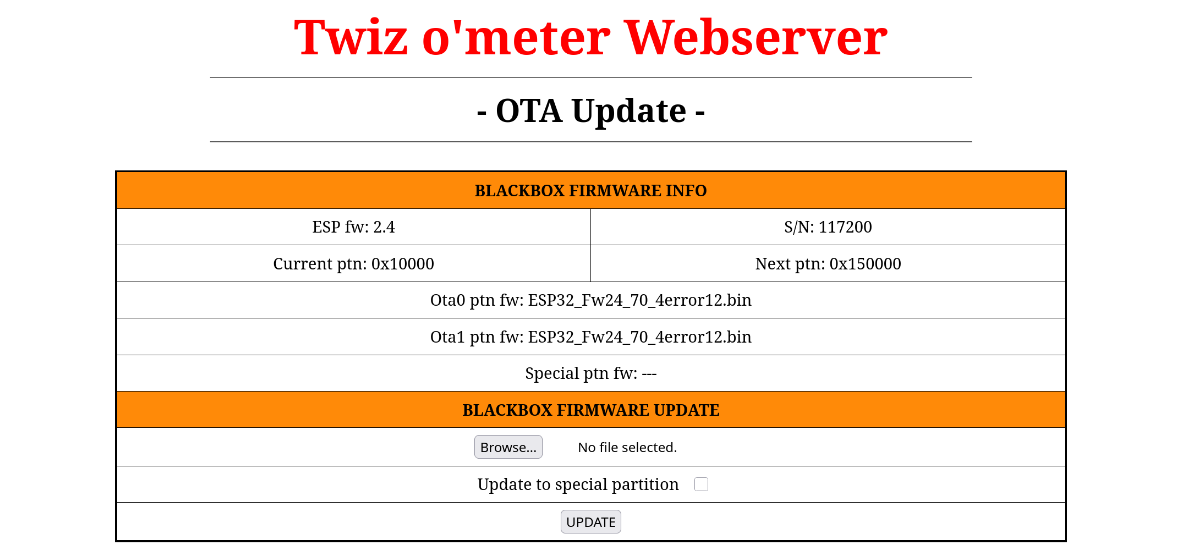
\includegraphics[width=1\textwidth]{figures/ota_page3.png}
    \caption{OTA-Update-Seite --- Update- und Informationstabelle.}
\end{figure}

Wenn der Fortschrittsbalken 100\% erreicht, wird das ToM+-LCD-Display schwarz.
Dies ist das erfolgreiche Zeichen dafür, dass ToM+ neu startet und die
\textit{Twizy-cfg}-Software lädt.
Verbinden Sie sich nun auf Ihrem Gerät mit dem Access Point \textbf{„Twizy-cfg“}, um auf
dessen Webserver zuzugreifen. Falls Sie dazu aufgefordert werden, bestätigen Sie,
dass die Verbindung aktiv bleiben soll, auch wenn kein Internetzugang verfügbar ist.

Das \textbf{Passwort} ist das Standard-ToM+-Passwort, also das Wort „pass“ gefolgt von der
Seriennummer Ihres Geräts (z.\,B. \textit{pass129777}). Die Seriennummer finden Sie auf der
Einstellungsseite, wie in Abbildung~\ref{fig:settings_page} erklärt.\\

Öffnen Sie nun einen Webbrowser und geben Sie \textbf{192.168.4.1/webserial} ein, um zum
Webserver-Interface zu gelangen, über das Sie Tuning-Befehle senden können.
Das Command-Terminal sieht ähnlich aus wie das hier gezeigte Bild.
Wie bereits erwähnt, ist Tuning keine offizielle ToM+-Funktion und
\textit{Twizy-cfg} wurde nicht von mir entwickelt. Informationen zu Tuning-Befehlen und
Konfigurationen finden Sie daher im \href{https://www.twizy-forum.de/projekte-twizy/83451-twizy-cfg-sevcon-shell-fuer-arduino?start=0}{Twizy-cfg-Forumsthema}
oder im \href{https://github.com/dexterbg/Twizy-Cfg}{Github-Repository}.\\

\begin{figure}[H]
    \centering
    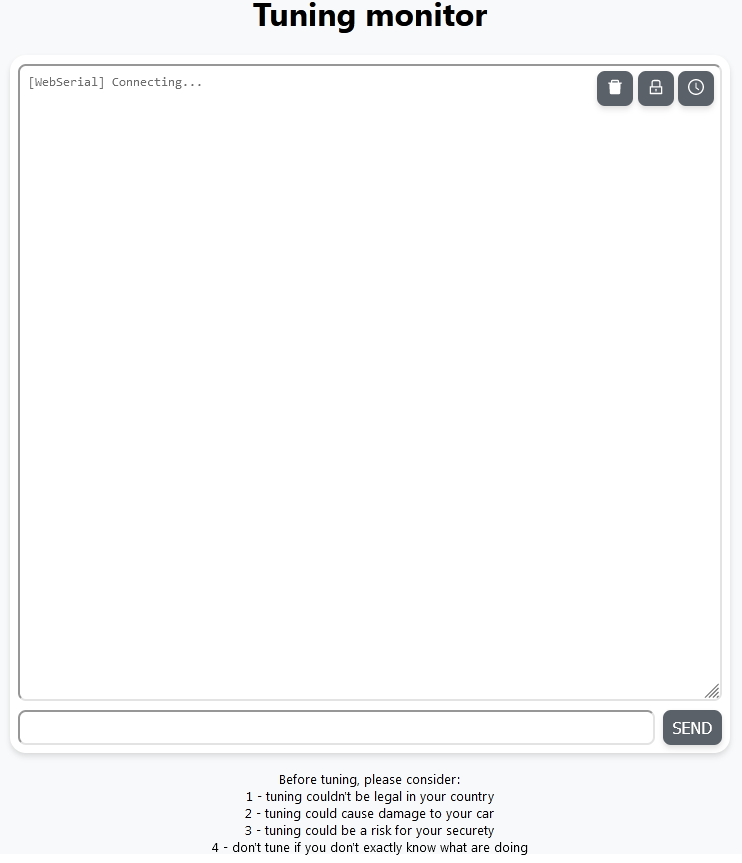
\includegraphics[width=0.7\textwidth]{figures/TuningMonitor.PNG}
    \caption{Tuning-Monitor zur Ausführung von Tuning-Befehlen.}
\end{figure}

Solange Sie Twizy-cfg verwenden, wird die ToM+-Firmware nicht geladen und das Display
bleibt daher ausgeschaltet. Wenn Sie zur offiziellen ToM+-Firmware zurückkehren möchten,
müssen Sie lediglich den selbsterklärenden Befehl \textbf{reboot} im Tuning-Monitor eingeben.\\

Damit startet ToM+ neu und wechselt zur anderen Partition, sodass es wieder sein normales
Verhalten zeigt. Die Tuning-Konfiguration bleibt dabei in Ihrem Twizy erhalten.
Wenn Sie die Twizy-cfg-Shell erneut benötigen, öffnen Sie einfach die Seite
\textbf{„OTA Update and Prefs“} auf dem ToM+-Webserver und wählen Sie die Option
\textit{„REBOOT FROM SPECIAL PARTITION“} aus der in der folgenden Abbildung gezeigten Tabelle.
Die \textit{“.bin”}-Datei muss nicht erneut hochgeladen werden.

\begin{figure}[H]
    \centering
    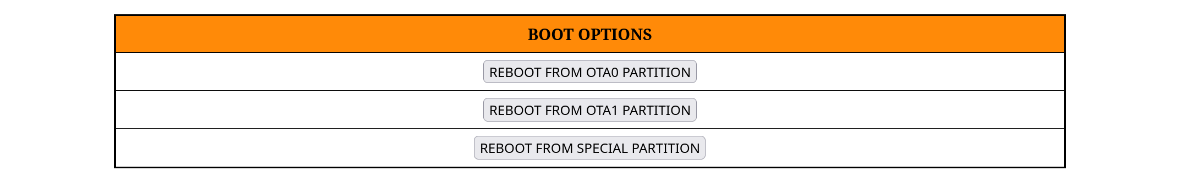
\includegraphics[width=1\textwidth]{figures/ota_boot.png}
    \caption{OTA-Update-Seite --- Tabelle mit Boot-Optionen.}
\end{figure}


\chapter{Steuerung eines Tasmota-WLAN-Schalters}
\label{apx:tasmota}

\section{Was sind WLAN-Schalter/-Steckdosen?}

In diesem Anhang erkläre ich, wie Sie Ihr ToM+ so konfigurieren können, dass es mit einem
WLAN-AC-Schalter / einer WLAN-AC-Steckdose oder jedem anderen Gerät mit
\textbf{Tasmota-Firmware} interagiert.

Im Grunde handelt es sich dabei um \textit{Relaismodule}, die über eine drahtlose Verbindung
aus der Ferne gesteuert werden können.
Solche Geräte sind auf vielen E-Commerce-Websites (wie Amazon) für wenige Dutzend Euro erhältlich.\\

Sie sind in vielen verschiedenen Bauformen erhältlich, häufig jedoch in den beiden in der Abbildung
gezeigten Varianten.
Die zweite Variante ist kompakter und benutzerfreundlicher, während die erste eine
Kabelverbindung benötigt, um mit Ihren elektrischen Geräten verbunden zu werden.

\begin{figure}[ht]
    \centering
    \begin{subfigure}[t]{0.48\textwidth}
        \centering
        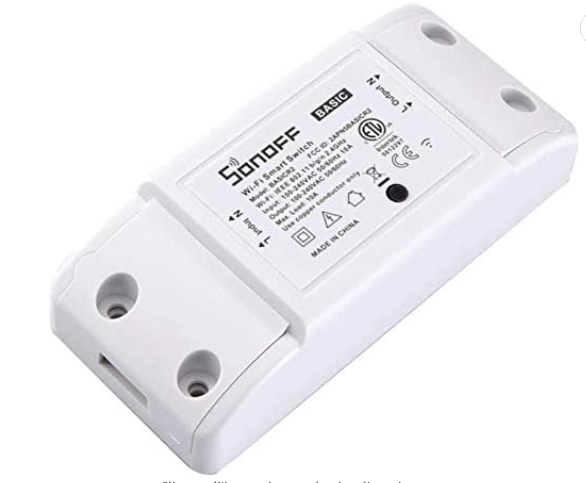
\includegraphics[width=\linewidth]{figures/Sonoff.PNG}
        \caption{Sonoff WLAN-Smart-Switch.}
    \end{subfigure}
    \hfill
    \begin{subfigure}[t]{0.48\textwidth}
        \centering
        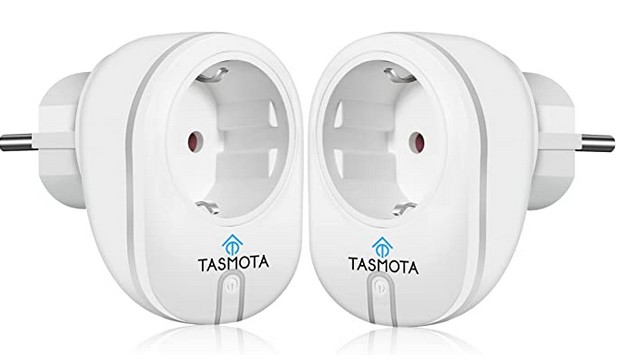
\includegraphics[width=\linewidth]{figures/TasmotaPlug.PNG}
        \caption{Tasmota-WLAN-Smart-Plug.}
    \end{subfigure}
\end{figure}

\textit{Aber warum ist das nützlich?} Es gibt viele Gründe, warum Sie ToM+ mit solchen Geräten
verbinden möchten.
Nehmen wir an, Sie möchten das Laden der Traktionsbatterie stoppen, wenn das Ladegerät überhitzt,
und den Ladevorgang wieder starten, wenn die Temperatur sinkt; oder Sie möchten
\textbf{den Ladevorgang stoppen}, sobald ein gewünschter SOC erreicht wurde.

Oder, wie ich es in diesem Anhang zu experimentellen Zwecken gemacht habe, eine Lampe in meinem
Zimmer einschalten, wenn der Twizy (in der Garage geparkt) den Ladevorgang fast abgeschlossen hat.
Kurz gesagt gibt es zahlreiche nützliche Ideen, bei denen ein WLAN-Schalter/eine WLAN-Steckdose
zusammen mit ToM+ eingesetzt werden kann, um interessante Projekte zu realisieren.


\section{Voraussetzungen}

Dafür benötigen Sie eine Blackbox mit einer Firmware-Version \textbf{1.4}
oder höher. Dies ist eine wichtige Voraussetzung, da dieser Vorgang Funktionen benötigt,
die mit der genannten Version eingeführt wurden. Siehe Abschnitt~\ref{sec:settings_page},
um Ihre ESP-Firmware-Version zu überprüfen, und Abschnitt~\ref{sec:web_ota_update}, um Ihre
Firmware bei Bedarf per OTA zu aktualisieren.

Zusätzlich müssen \textbf{WLAN und MQTT konfiguriert} sein, damit das gesamte System
funktioniert. Falls dies noch nicht geschehen ist, lesen Sie bitte Abschnitt~\ref{sec:wifi_settings},
um WLAN einzurichten, und Abschnitt~\ref{sec:mqtt_connection} für die MQTT-Konfiguration.
Beide müssen aktiviert und verbunden sein, damit diese Funktion verwendet werden kann.\\

Außerdem benötigen Sie selbstverständlich einen WLAN-Schalter oder eine WLAN-Steckdose,
je nach Bedarf. Das Gerät muss mit einer \textbf{Tasmota-Firmware} (\textit{Version 7} oder höher) laufen.

Beachten Sie, dass Geräte wie \textit{„Sonoff“} ab Werk mit einer proprietären Firmware ausgeliefert werden,
die das MQTT-Protokoll nicht nativ unterstützt.\\

Um solche Geräte wie in diesem Anhang verwenden zu können, müssen Sie sie auf die Tasmota-Firmware aktualisieren.
Im Internet finden sich zahlreiche Anleitungen zur Installation der Tasmota-Firmware.
Suchen Sie nach einer Anleitung, die zu Ihrem Gerät passt, und folgen Sie dieser.
Wenn Sie sich nicht mit dem Firmware-Update beschäftigen möchten, empfehle ich persönlich,
ein Gerät zu kaufen, auf dem Tasmota bereits installiert ist.


\section{Tasmota-MQTT-Konfiguration}

Navigieren Sie zur \textbf{Tasmota WebUI}. Dort wird eine Startseite ähnlich der unten gezeigten angezeigt.
Bei Unsicherheiten können Sie jederzeit die \href{https://tasmota.github.io/docs/}{offizielle Dokumentation}
konsultieren.

\begin{figure}[H]
    \centering
    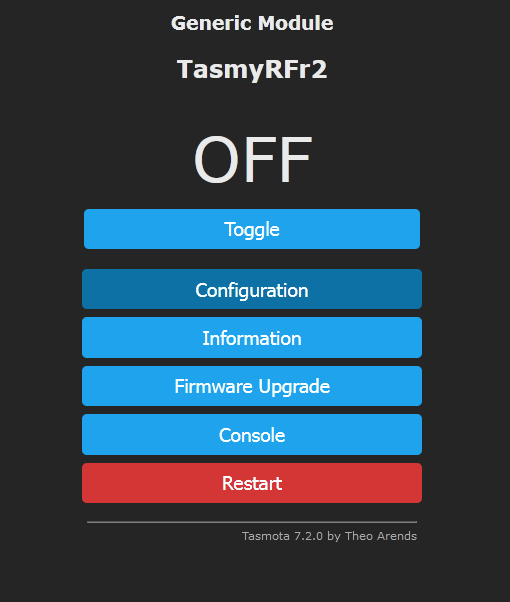
\includegraphics[width=0.45\textwidth]{figures/Mqtt1.PNG}
    \caption{Tasmota WebUI --- Startseite.}
\end{figure}

Drücken Sie zunächst die Schaltfläche \textbf{„Configuration“}, die Sie zur auf dem ersten Bild
unten gezeigten Seite führt.
Konfigurieren Sie anschließend die \textit{WLAN-Verbindung}, indem Sie Ihre Zugangsdaten
(SSID und Passwort) auf der Tasmota-Seite \textbf{„Configure WiFi“} eingeben.
Folgen Sie danach den Anweisungen zur Konfiguration der
\textit{MQTT-Einstellungen}, indem Sie die WebUI-Seite \textbf{„Configure MQTT“} aufrufen.\\

\clearpage

\begin{figure}[ht]

    \begin{subfigure}[t]{0.4\textwidth}
        \centering
        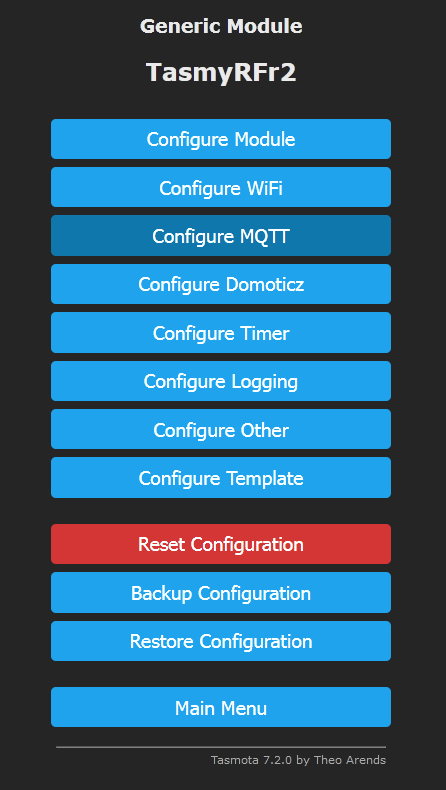
\includegraphics[width=\linewidth]{figures/Mqtt2.PNG}
        \caption{Konfigurationsseite.}
    \end{subfigure}
    \hfill
    \begin{subfigure}[t]{0.48\textwidth}
        \centering
        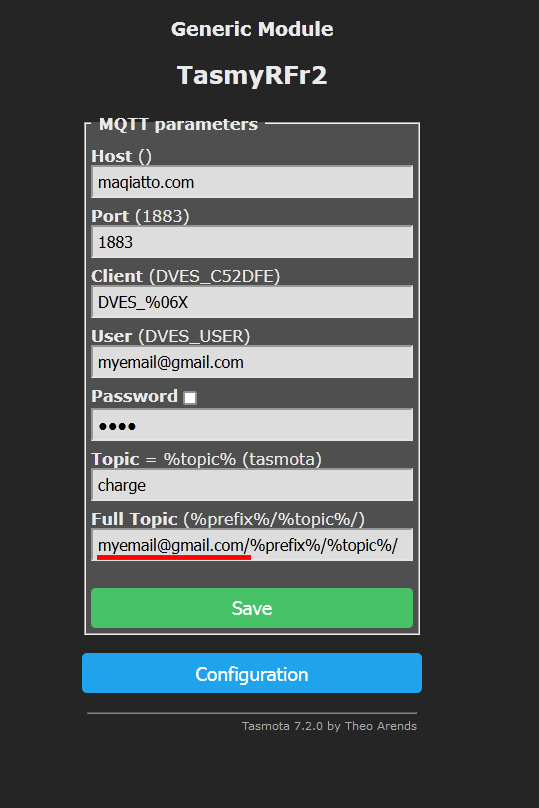
\includegraphics[width=\linewidth]{figures/Mqtt4.PNG}
        \caption{MQTT-Konfigurationsseite.}
    \end{subfigure}
\end{figure}

Geben Sie nun Broker-Adresse, Benutzer-ID, Passwort und Portnummer ein.
Diese müssen mit den auf ToM+ eingestellten Werten übereinstimmen!
Die Erklärung der einzelnen Felder finden Sie in Abschnitt~\ref{sec:mqtt_connection}.\\

Die schwierigsten Parameter sind \textbf{„Topic“} und \textbf{„Full Topic“}.
Diese dürfen nicht mit den MQTT-Topics von ToM+ identisch sein, da sie spezifisch für das von Ihnen
verwendete Gerät sind.
Wenn Sie dieselben \textit{TOMin}- und \textit{TOMout}-Topics verwenden, können sich die
Kommunikationen gegenseitig stören.\\

Geben Sie im ersten Feld einen beliebigen Wert ein.
Ich empfehle eine kurze Bezeichnung, die an die Funktion Ihres Geräts erinnert.
Verwenden Sie jedoch eine kurze Zeichenfolge (5/6 Zeichen sind ausreichend), da dieses Feld nur
einen kleinen Teil des vollständigen Topic-Strings bildet und ToM+ eine Begrenzung von 50 Zeichen
für das Feld \textbf{„Auxilliary MQTT command“} besitzt (siehe Abschnitt~\ref{sec:web_alarm_triggers}).\\

Beim zweiten Feld ist es wichtig, zwischen zwei Optionen zu unterscheiden, abhängig davon,
welchen Broker Sie verwenden.
Wenn Sie einen eigenen Broker verwenden (also \textit{nicht Maqiatto}), lassen Sie die
Standardzeichenfolge \textbf{\%prefix\%/\%topic\%/} unverändert.\\

Wenn Sie stattdessen Maqiatto verwenden, das gemäß Abschnitt~\ref{sec:free_broker} konfiguriert wurde,
oder einen anderen Broker, der \textit{Ihre E-Mail-Adresse als Präfix} des Topic-Namens hinzufügt,
bearbeiten Sie das Feld \textbf{„Full Topic“} entsprechend.
Die Felder sehen dann wie im zweiten Bild oben aus, sodass \linebreak
\textbf{myemail@gmail.com/\%prefix\%/\%topic\%/} eingetragen wird,
wobei Ihre Benutzer-ID (E-Mail-Adresse) als Präfix hinzugefügt wird.

Drücken Sie abschließend die grüne Schaltfläche \textbf{„Save“} und warten Sie, bis das Gerät neu startet.\\

\textbf{NICHT VERGESSEN!} Wenn Sie den Maqiatto-Broker verwenden, müssen Sie möglicherweise
das neue Topic zu Ihrem Konto hinzufügen, wie in Abbildung~\ref{sec:free_broker_add_topics} erklärt.

In diesem Fall müssen Sie \textbf{cmnd/<your\textunderscore~Tasmota\textunderscore~topic\textunderscore~name>/Power}
als neuen Topic-Namen hinzufügen.
Wenn Sie dem Beispielbild gefolgt sind, lautet dieser \textit{cmnd/charge/Power}.


\section{ToM+-Tasmota-Konfiguration}

Öffnen Sie den ToM+-Webserver wie in Abschnitt~\ref{sec:web_server_access} beschrieben und gehen Sie zur
Seite \textbf{„Alarm triggers“}.
Fügen Sie nun einen neuen Alarm zur Liste hinzu, entsprechend dem Wert, der Ihr Tasmota-Gerät
steuern soll, wie in Abschnitt~\ref{sec:web_alarm_triggers} beschrieben.

In meinem Fall habe ich den Wert \textbf{„Battery SOC“} gewählt, der einen Alarm auslöst,
wenn sein Wert \textit{97\%} erreicht, um den fast abgeschlossenen Ladevorgang zu melden.

\begin{figure}[H]
    \centering
    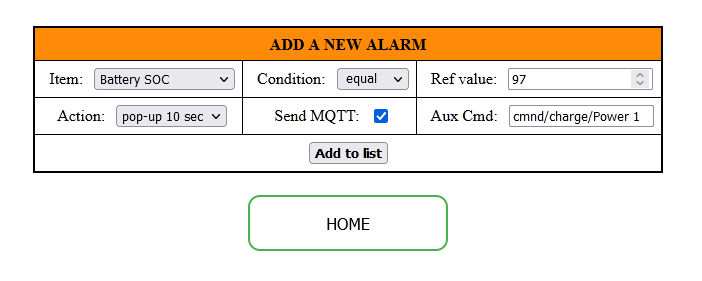
\includegraphics[width=0.7\textwidth]{figures/Tom01.PNG}
    \caption{Hinzufügen des Tasmota-Triggers in ToM+.}
\end{figure}

Wie Sie sehen können, ist der wichtigste Teil die korrekte Konfiguration des Feldes
\textbf{„Aux Cmd“}, da es den MQTT-Steuerbefehl enthält, den ToM+ an das
Tasmota-Gerät senden wird.

Wenn Sie einen eigenen MQTT-Broker verwenden (also \textit{nicht Maqiatto}), hat
\textbf{Aux Cmd} folgende Syntax:
\begin{itemize}
    \item \textit{cmnd/<your\textunderscore~Tasmota\textunderscore~topic\textunderscore~name>/Power 1}, wenn das Gerät eingeschaltet werden soll.
    \item \textit{cmnd/<your\textunderscore~Tasmota\textunderscore~topic\textunderscore~name>/Power 0}, wenn das Gerät ausgeschaltet werden soll.
\end{itemize}
In unserem Beispiel lautet der Befehl zum Einschalten der Lampe \textbf{cmnd/charge/Power 1}.\\

Wenn Sie hingegen den Maqiatto-Broker oder einen anderen Broker verwenden, der Ihre Benutzer-ID (E-Mail-Adresse)
als Präfix im Topic-Namen verwendet, sieht die Syntax für \textbf{Aux Cmd} folgendermaßen aus:
\begin{itemize}
    \item \textit{myemail@gmail.com/cmnd/<your\textunderscore~Tasmota\textunderscore~topic\textunderscore~name>/Power 1}, um das Gerät einzuschalten.
    \item \textit{myemail@gmail.com/cmnd/<your\textunderscore~Tasmota\textunderscore~topic\textunderscore~name>/Power 0}, um das Gerät auszuschalten.
\end{itemize}
In unserem Fall lautet der Befehl \textbf{myemail@gmail.com/cmnd/charge/Power 1}.\\

Wenn Sie den Ladevorgang stoppen und anschließend unter bestimmten Bedingungen wieder starten möchten,
müssen Sie zwei Alarme hinzufügen: einen für die Power-ON- und einen für die Power-OFF-Bedingung,
jeweils mit der oben beschriebenen Syntax.\\

Bitte beachten Sie, dass Sie bei einem Gerät mit mehreren Relais die oben beschriebene Syntax
anpassen müssen, um festzulegen, welches Relais Sie steuern möchten:
Verwenden Sie \textbf{„Power1“} für das erste Relais, \textbf{„Power2“} für das zweite und so weiter.
Dies ergibt:
\begin{itemize} 
    \item \textit{cmnd/<your\textunderscore~Tasmota\textunderscore~topic\textunderscore~name>/Power1 1}, um das erste Relais einzuschalten.
    \item \textit{cmnd/<your\textunderscore~Tasmota\textunderscore~topic\textunderscore~name>/Power1 0}, um es auszuschalten.
\end{itemize}
Die gleiche Unterscheidung bezüglich Maqiatto und eigenen Brokern gilt auch hier.


\section{Häufige Probleme und Lösungen}

Einige Tasmota-Firmwares kommen mit dem \textit{Maqiatto}-Topic-Format nicht gut zurecht.
Wenn Sie ein Tasmota-Gerät mit ToM+ steuern möchten, müssen Sie daher einen anderen MQTT-Broker verwenden.
Nach einigen Tests habe ich festgestellt, dass Sie erfolgreich \href{https://dealgate.ru/}{mqtt.dealgate.ru}
verwenden können, einen kostenlosen und funktionsreicheren Broker.

Der Nachteil ist, dass Sie bei der Erstellung des Kontos mit einigen russischen Übersetzungen
konfrontiert werden.
Aber dafür reicht ein Online-Übersetzer problemlos aus.
